\documentclass[12font]{article}
\title{\textbf{ Time-Reversal Symmetry and Majorana Correlators }}
\author{Chen-Chih Wang  }
\date{\textit{Department of physics, National Tsing Hua University, Hsinchu 30013, Taiwan} \\ (Dated: \today)}
\usepackage[margin=2cm]{geometry}
%\usepackage[fleqn]{amsmath}
%\usepackage{CJK,amsmath}
\usepackage{amsfonts,amssymb}
\usepackage{fancyhdr}
%\pagestyle{fancy}
\usepackage{textcomp}
\usepackage{graphicx}
\usepackage{float}
\usepackage{color}
\usepackage{tikz}
\usepackage{multicol}
\usepackage{threeparttable}
\usepackage{amsthm}
\usepackage{mathtools}
\usepackage{hyperref}
\urlstyle{same}
\usepackage{caption}
\usepackage{subcaption}
\usepackage{dsfont}
\usepackage{comment}
\newtheorem{theorem}{Theorem}[section]
\theoremstyle{definition}
\newtheorem{definition}{Definition}[section]
\newtheorem{lemma}[theorem]{Lemma}
\newtheorem{corollary}{Corollary}[theorem]
\newtheorem{proposition}[theorem]{Proposition}

\numberwithin{equation}{section}

\newcommand{\vac}{\mrm{vac}}
\newcommand{\Bra}[1]{\left\langle #1 \right|}
\newcommand{\Ket}[1]{\left| #1 \right\rangle}
\newcommand{\bra}[1]{\langle #1 |}
\newcommand{\ket}[1]{| #1 \rangle}
\newcommand{\anglelr}[1]{\left\langle #1 \right\rangle}
\newcommand{\sanglelr}[1]{\langle #1 \rangle}
\newcommand{\braket}[2]{\langle #1 | #2 \rangle}
\newcommand{\Bbraket}[2]{\left\langle #1 \right|\left. #2 \right\rangle}
\newcommand{\dif}[1]{\frac{\mathrm{d}}{\mathrm{d}#1}}
\newcommand{\diff}[2]{\frac{\mathrm{d}#1}{\mathrm{d}#2}}
\newcommand{\gd}{\boldsymbol{\nabla}}
\newcommand{\dive}{\boldsymbol{\nabla}\cdot}
\newcommand{\curl}{\boldsymbol{\nabla}\times}
\newcommand{\lr}[1]{\left(  #1  \right)}
\newcommand{\lrm}[1]{\left[  #1  \right]}
\newcommand{\lrg}[1]{\left\{  #1  \right\}}
\newcommand{\abs}[1]{\left|  #1  \right|}
\newcommand{\de}{\partial}
\newcommand{\pdif}[1]{\frac{\partial}{\partial#1}}
\newcommand{\pdiff}[2]{\frac{\partial#1}{\partial#2}}
\newcommand{\mrm}[1]{\mathrm{#1}}
\newcommand{\bo}[1]{\mathbf{#1}}
\newcommand{\bog}[1]{\boldsymbol{#1}}
\newcommand{\vint}[3]{\int_{#1}#2\cdot\mathrm{d}\mathbf{#3}}
\newcommand{\voint}[3]{\oint_{#1}#2\cdot\mathrm{d}\mathbf{#3}}
\newcommand{\Vint}{\int\mrm{d}^3\bo{r}'}
\newcommand{\rr}{\mathbf{r} - \mathbf{r}'}
\newcommand{\arr}{\left|\mathbf{r} - \mathbf{r}'\right|}
\newcommand{\nx}{\hat{\bo{n}}_1}
\newcommand{\ny}{\hat{\bo{n}}_2}
\newcommand{\alert}[1]{{\color{red}#1}}
\newcommand{\alertV}[1]{{\color{violet}#1}}
\newcommand{\Tr}{\mrm{Tr}}
\newcommand{\norm}[1]{\left\lVert#1\right\rVert}

\newcommand{\wordfig}[2]{\begin{minipage}[h]{#1 cm}
	\vspace{0pt}
	\includegraphics[width=\textwidth]{#2}
   \end{minipage}}

\begin{document}
\maketitle
%\fontsize{12pt}{18pt}\selectfont

\begin{figure}[H]
  \centering
  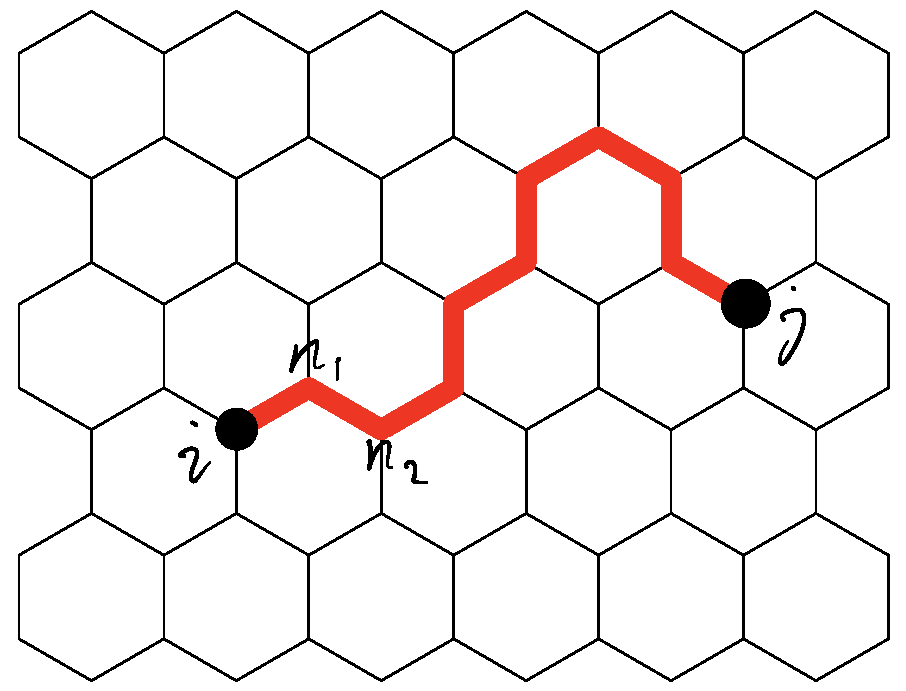
\includegraphics[width=0.3\textwidth]{String}
  \caption{The configuration $\mathcal{M}$ contains only one single string. Points $i$ and $j$ are the end points of the sting, and $n_1,n_2,\cdots$ are the points in the middle}\label{String.f}
\end{figure}
Define the string operator
\[
\mathfrak{S}_\mathcal{M} := \prod_{\anglelr{kl}}\sigma^{\alpha_{kl}}_k\sigma^{\alpha_{kl}}_l
\]
and represent the Pauli algebra $[\sigma^\mu,\sigma^\nu] = 2i\epsilon^{\mu\nu\lambda}\sigma^\lambda$ using the Majorana operators in the way that $\sigma^\mu = \mathcal{P}_Gib^\mu c\mathcal{P}_G$ after the Gutzwiller projection, we then get
\[
\mathfrak{S}_\mathcal{M} = \mathcal{P}_G\lr{\prod_{\anglelr{kl}\in\mathcal{M}}\hat{u}_{kl}} \prod_{\anglelr{kl}\in\mathcal{M}}ic_kc_l\mathcal{P}_G = (-1)^{\abs{\mathcal{M}}\lr{\abs{\mathcal{M}}-1}/2} i^{\abs{\mathcal{M}}}\mathcal{P}_Gc_ic_j \prod_{\anglelr{kl}\in\mathcal{M}}\hat{u}_{kl}\mathcal{P}_G
\]
Where $i$ and $j$ are the end points of the string $\mathcal{M}$ illustrated in Fig.\ref{String.f}. $\abs{\mathcal{M}}$ stands for the length of the string. 

The length of the string is related to the TRS property of the string operator. If $\abs{\mathcal{M}}$ is an odd(even) number, then there will be an even(odd) number of middle points, i.e. points labeled by $n$ in FIg.\ref{String.f}, and then the string operator will be time-reversal even(odd). For $\abs{\mathcal{M}}$ being odd, the simplest example is the single bond, which consists of two spin operators. For $\abs{\mathcal{M}}$ being even, let's think of a sting consisting of two adjacent bonds, the string operator is then 
\[
\lr{\sigma_i^{x}\sigma_{n_1}^x}\lr{\sigma_{n_1}^y\sigma_{j}^y} = i\sigma_i^{x}\sigma_{n_1}^z\sigma_{j}^y
\]
(w.o.l.g we have assumed $\alpha_{i,n_1} = x$ and $\alpha_{n_1,j} = y$) The ground state $\ket{\psi}$ of the Kitaev model is time reversal invariant $\ket{\mathcal{T}\psi} = \ket{\psi}$. So, the expectation value of any time-reversal odd quantity has to be zero. Therefore, the expectation value of the string operator with $\abs{\mathcal{M}} = 2$ has to be zero
\[
\anglelr{\lr{\sigma_i^{x}\sigma_{n_1}^x}\lr{\sigma_{n_1}^y\sigma_{j}^y}} = i\anglelr{\sigma_i^{x}\sigma_{n_1}^z\sigma_{j}^y}
\]
because the operator $\sigma_i^{x}\sigma_{n_1}^z\sigma_{j}^y$ is time-reversal odd. Based on this logic one can get the corollary that \emph{the expectation value of string operators with an even number of $\abs{\mathcal{M}}$ must be zero in any state preserving TRS.}

Because $[\hat{u}_{ij},\hat{H}] = 0$, we know the Kitaev ground state is an eigenvector of the gauge field operator $\hat{u}_{ij}$ after fixing the gauge. Denote by $\ket{\psi_0} = \ket{u}\ket{M}$ the Kitaev ground state with gauge field fixed ($\ket{u}$ can be arbitrary, it has not to be all-positive gauge). Then, the expectation value of the string operator can be evaluate in the gauge-fixed Majorana space,
\[
\anglelr{\mathfrak{S}_\mathcal{M}} = 0 = \underbrace{(-1)^{\abs{\mathcal{M}}\lr{\abs{\mathcal{M}}-1}/2} i^{\abs{\mathcal{M}}} \bra{u}\lr{\prod_{\anglelr{kl}\in\mathcal{M}}\hat{u}_{kl}}\ket{u}}_{\neq 0} \bra{M}c_ic_j\ket{M}
\]
So consequently, we then immediately get another result that \emph{$\anglelr{c_ic_j} = \bra{M}c_ic_j\ket{M}$ in the Kitaev ground state must be zero if $i$ and $j$ are the end points of a string $\mathcal{M}$ with an even number of length $\abs{\mathcal{M}}$}. 

In summary, the fact that the Majorana correlator $\anglelr{c_ic_j}$ is zero if $i$ and $j$ belong to the same type of sublattice (reflecting the string length to be even or odd) relies on only three conditions,
\begin{itemize}
  \item TRS states (don't need to be the ground state)
  \item $[\hat{u}_{ij},\hat{H}] = 0$.
  \item $b$-sector can be perfectly separated from $c$-sector in the theory.
\end{itemize}

\end{document}